\chapter{BoBshield API}
\label{kap:3}

\section{API pre MATLAB}
\label{kap:3.1}
MATLAB je programovacie a výpočtové prostredie, využívané širokou škálou technikov a vedcov na numerické výpočty, modelovanie, analýzu dát a ich interpretáciu, návrhy algoritmov, simuláciu a riadenie systémov. Názov vznikol skrátením anglického výrazu Matrix Laboratory, z čoho vyplýva, že základom pri výpočtoch je práve práca s maticami. Jeho využitie má veľmi široký záber a jeho uplatnenie vieme nájsť aj pri robotike alebo umelej inteligencii. Vďaka širokému spektru toolboxov a balíkov voľne dostupných na platformách ako je Github sa jeho obzory stále zväčšujú. MATLAB je pre univerzity a študentov voľne dostupný, preto je medzi študentami s technickým zameraním veľmi populárny a často využívaný. Aby si študenti mohli vyskúšať automatické riadenie systému gulička na tyči (Ball on Beam) je potrebné vytvoriť k nášmu hardware aj príslušné API pre daný software.  

\subsection{Tvorba API pre MATLAB}
\label{kap:3.1.1}

\subsection{Knižnica pre snímač}
\label{kap:3.1.2}

\subsection{Funkcie}
\label{kap:3.1.3}

\subsection{Príklady}
\label{kap:3.1.4}

\section{API pre Simulink}
\label{kap:3.2}

\subsection{Knižnica}
\label{kap:3.2.1}

\subsection{Príklady}
\label{kap:3.2.2}

\section{API pre Arduino IDE}
\label{kap:3.3}

Pri meraniach presnosti ToF snímača pre rôzne materiály, povrchy a farby guličiek sme mohli pozorovať šum, ktorý nám pri nameraných hodnotách vznikal. Hoci tento nežiaduci jav nie je možné celkom odstrániť, môžeme jeho dopad na namerané hodnoty výrazne znížiť pomocou implementácie jednoduchej filtrácie nameraných hodnôt vhodnou metódou.
Pre našu aplikáciu sme testovali 2 typy filtrácia a to pomocou aritmetického priemeru a váženého priemeru. Pri testovaní sme postupovali nasledovne. Základom bolo získanie súboru nameraných hodnôt, na ktorý budeme môcť aplikovať obidva filtre a následne navzájom porovnať ich výstupy. Vstup je pre oba typy filtrov identický a preto môžeme spoľahlivejšie rozhodnúť o tom, ktorý z filtrov si zvolíme. Tieto hodnoty vstupu sme získali meraním polohy guličky pri jej posune z jednej koncovej polohy trubičky k druhej, pri minimálnom naklonení trubičky. 
Pri aritmetickom priemere sme z určitého počtu nameraných hodnôt urobili aritmetický priemer a výstupom bola 1 hodnota, z čoho vyplýva, že frekvencia, s ktorou sme merali je násobne väčšia ako frekvencia, získavania filtrovaných hodnôt. To môže mať za následok spomalenie systému z hľadiska rýchlosti reakcie na zmenu polohy guličky. Vlastnosti daného typu filtráciu vieme ovplyvniť počtom nameraných hodnôt, z ktorých robíme aritmetický priemer. Zvyšovanie počtu hodnôt má za následok zlepšenie filtrácie a väčšie vyhladenie vstupu, no zároveň spôsobuje spomalenie systému, čo môže byť pozorované hlavne keď gulička rýchlo mení svoju polohu. 
Vážený priemer je založený na princípe zberu a ukladaní určitého počtu hodnôt, pričom pri každom ďalšom meraní sa nám najstaršia hodnota vymaže a pozíciu prvej hodnoty zaujme najnovšie nameraná hodnota. Z tohto súboru hodnôt sa nám pri každom meraní vypočíta vážený priemer, teda frekvencia merania a frekvencia získavania nameraných hodnôt je identická. Ako vyplýva z názvu, každá hodnota má inú váhu, teda rozdielny vplyv na výslednú hodnotu.  Výsledná hodnota sa následne vypočíta podľa nasledujúceho vzorca:


\begin{align}
	\label{rovnica.3.3.1}
	priemer = \sum_{i=1}^{N}x_i*p(x_i)= x_1*p(x_1)+x_2p(x_2)+\cdots +x_N*p(x_N)
\end{align}

Vlastnosti filtrácie teda vieme ovplyvňovať jednak počtom hodnôt, z ktorých váhovaný priemer robíme, ale aj zmenou parametrov ovplyvňujúcich váhu jednotlivých hodnôt, teda vplyv na výsledok.

Vzorku hodnôt, na ktorej sme porovnávali vplyv jednotlivých typov filtrov sme si vykreslili do grafu v prostredí MATLAB spolu s grafmi hodnôt získaných po aplikácii filtrov. Následne sme menili parametre filtrov, či už išlo o počet hodnôt, z ktorých sme tvorili priemer alebo pri váhovanom priemer, o nastavenie parametrov váhovania.

\begin{figure}[!h]
	\centering
	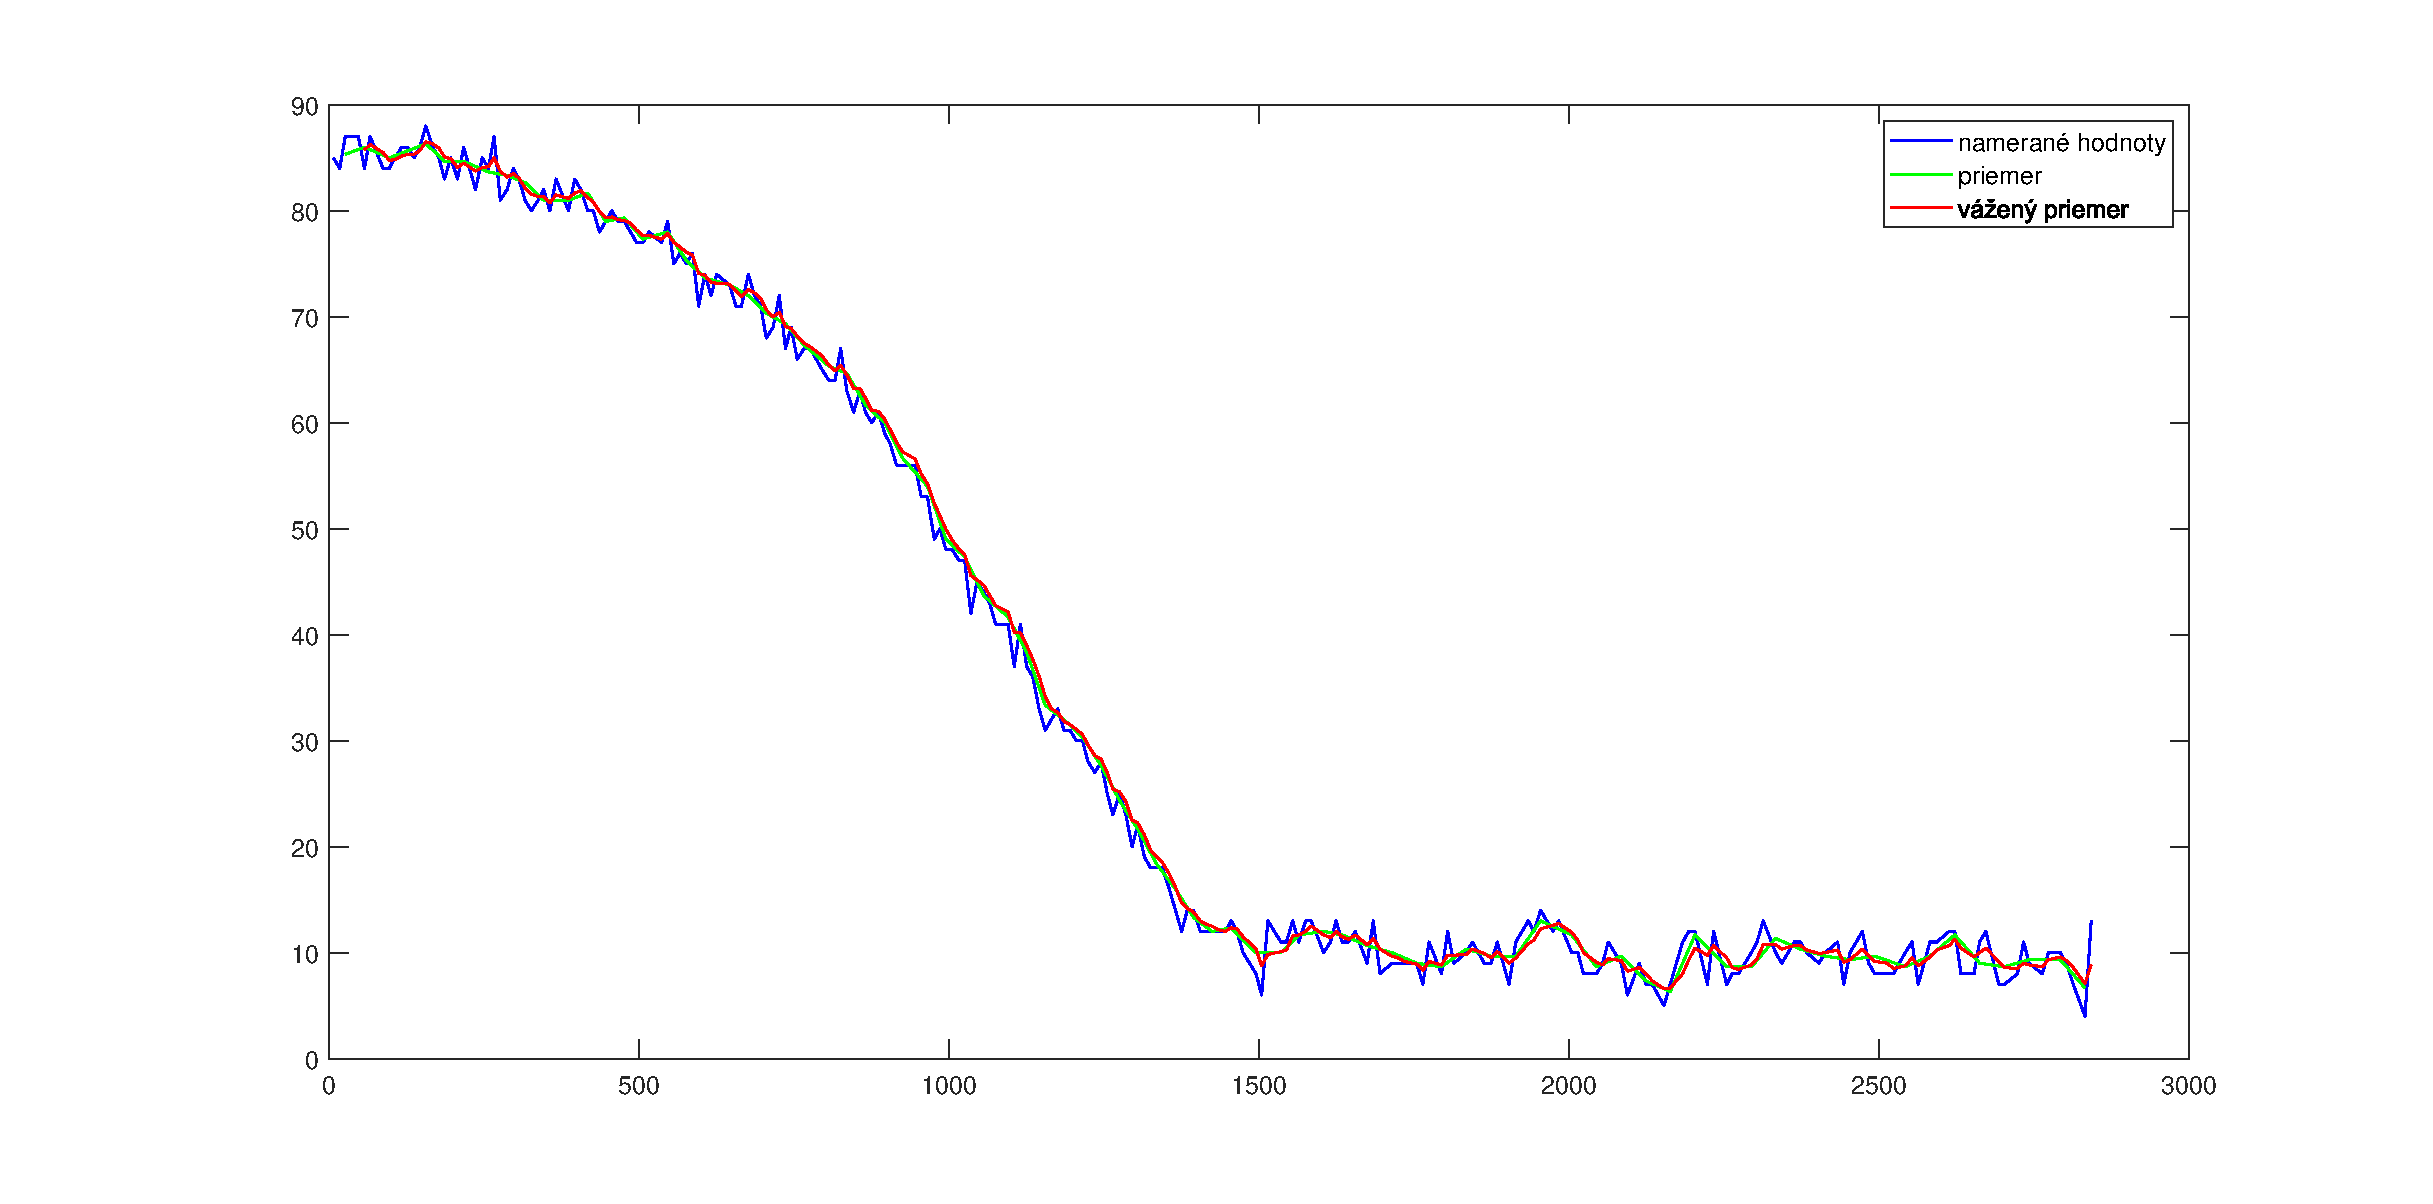
\includegraphics[width=140mm]{obr/Filtracia.eps}
	\caption{Porovnanie jednotlivých typov filtrácií }\label{OBRAZOK 3.3.1} 
\end{figure} 

Na obrázku \ref{OBRAZOK 3.3.1} môžeme vidieť porovnanie 2 typov filtrov, ktoré sme testovali, spolu s pôvodnými, nefiltrovanými nameranými hodnotami. 
Pre náš systém sme sa rozhodli použiť pre filtráciu šumu vážený priemer z 5 hodnôt s váhou jednotlivých parametrov: $p_1=4, p_2=3, p_3=2, p_4=2, p_5=1$.
Vyhladenie šumu je veľmi podobné pri oboch filtroch, v čom je pre nás však vážený priemer výhodnejší, je práve získavanie filtrovaných hodnôt s násobne väčšou frekvenciou.

